\section{A generic model-code synchronization pattern}
\label{sec:processes}
This section describes our generic artifact synchronization methodology pattern. 
%Although, the pattern is presented in a model-code synchronization-oriented way, it is flexibly extensible to any artifacts. 
For the sake of generality, we postulate that the architect and programmer are actors with starkly opposite development practices.
This allows the approach to be used even in cases where model
and code can both be used for the full implementation of a system,
rather than just architectural design for the former,
and code implementation for the latter.

\subsection{Definitions}
\label{sec:use-case}

In this section we define the actors who will use our model-code synchronization approach to collaborate during development.
%Then we define the main capabilities, as use-cases, expected from a generic IDE used by these actors.
Some basic concepts related to the actors and use-cases are also defined in this section.


%\subsection{Collaborating actors and development artifacts}

%In this paper we propose a methodological model-code synchronization pattern for collaboration between software
%architects and programmers.

First, we introduce the concepts of \textit{development artifact} and \textit{baseline artifact}.

\begin{definition}[Development artifact]
	A development artifact is an artifact, as defined in \cite{omg_software_2008},
	that can be used for the full implementation of the system.
\end{definition}

%For example a system can be entirely implemented as code.
%Implementation code is a development artifact, so may model.
%It is then not only documentation of specification
%but part of the implementation.
%For example a model can be used for implementation by generating code from the model, and compiling the code without the need to edit or complete the code.
In our work, we assume that model and code are both development artifacts.
A development artifact may be the baseline artifact, defined in this paper as follows:

\begin{definition}[Baseline artifact]
	A baseline artifact is one which may be edited manually.
	All other artifacts are produced from the baseline artifact
	through some process, and only through a process. Manual edition
	of artifacts other than the baseline artifact is forbidden.
\end{definition}

Two primary actors, called \textit{model-driven developer}
and \textit{code-driven developer}, are introduced.
%The main difference between them
%is what they consider as the baseline artifact.

\begin{definition}[Model-driven developer]
	A model-driven developer is an actor in a software development process
	for whom the baseline artifact is the model.
\end{definition}

%In other words, for the model-driven developer only the model should be edited manually. 
The code must always be produced from the model automatically
by some process that guarantees that the code is consistent with the model.
A software architect is a kind of the model-driven developer
who edits the model to specify the architecture of the system.
%An architect presumes that the reference for the architecture
%of the system should be specified as a model.

\begin{definition}[Code-driven developer]
	Code-driven developer is an actor in a software development process
	for whom the code is the baseline artifact.
\end{definition}

A programmer is a specialization of the code-driven developer.
Indeed, programmers may modify the code, such as editing method bodies.
%The code is then the main reference for the implementation of methods.

There are some use-cases for manual edition of artifacts. The \texttt{Edit Artifact} use-case
implies that the IDE must have some tool to let the developer manually edit an artifact.
The \texttt{Edit Model} and \texttt{Edit Code} use-cases are specializations of the \texttt{Edit Artifact}
use-case where the artifact is the model or code.

There are also some use-cases related to the synchronization of artifacts. The \texttt{Synchronize Artifact} use-case (1) compares two artifacts, (2) updates each with editions made
in the related artifact, and (3) reconciles conflicts when appropriate. The \texttt{Synchronize Model} and \texttt{Synchronize Code}
use-cases are specializations where, respectively, the model or the code are the artifacts being synchronized.

The \texttt{Generate Code} use-case is related to forward engineering.
It is the production of code in a
programming language from a model.
The developer can either use \texttt{Generate Code (Batch)} or \texttt{Generate Code (Incremental)}.
%\end{comment}

\begin{definition}[Batch code generation \cite{Giese2006}]
	Batch code generation is a process of generating code
	from a model, from scratch.
	Any existing code is overwritten by the newly generated code.
\end{definition}

Incremental code generation is a specialization of incremental model transformation, which
is defined in \cite{Giese2006} as model transformation that
does not generate the whole target model from scratch but only updates the target model by
propagating editions made in the source model.

%\texttt{Incremental code generation (ICG)} \ti{$gen_{inc}$ is a process of taking as input a changed model m and an existing executable code to make the code synchronized with the changed model: $gen_{inc}(m, c) = c'$. Non-conflicted changes at the code side are kept intact the synchronization. ICG is also defined as a process of taking model changes ch and an existing code c: $gen_{inc}(ch, c) = c'$}.

%Derived from the definition of incremental model transformation, 
Incremental code generation
is defined in this paper as follows:

\begin{definition}[Incremental code generation]
	In-cremental code generation is the process
	of taking as input an edited model, and existing code, and then updating the code by propagating
	editions in the model to the code.
\end{definition}

%\begin{comment}
Finally, the \texttt{Reverse Code} use-case is related to reverse engineering.
\texttt{Reverse Code} is the production of a model, in a modeling language, from code, written in a programming language.
The developer can either use \texttt{Reverse Code (Batch)} or \texttt{Reverse Code (Incremental)}, which are defined in this paper as follows:
%\end{comment}

\begin{definition}[Batch reverse engineering]
	Batch reverse engineering is a process of producing a model from code, from scratch.
	The existing model is overwritten by the newly produced model.
\end{definition}

\begin{definition}[Incremental reverse engineering]
	Incremental reverse engineering is the process of taking as
	input a edited code, and an existing model, and then updating the model by propagating
	editions in the code to the model.
\end{definition}

%For readability, in this paper we will sometimes designate batch and incremental as modes
%of code generation/reverse; e.g. we say that we generate code in batch mode from a model.

%The use-cases are generic. They do not depend
%on any particular approach or tool. Therefore the software developers
%can choose the approach or tool that suits better his/her
%development preferences best.

In the next section, the use-cases of the IDE are integrated into
a process that covers model-code synchronization.
%The scenarios correspond to behaviors performed by both kinds of actors,
%i.e. model-driven developers and code-driven developers.

%Model-driven engineering has been established as a potential approach to gain software quality and productivity \cite{Mussbacher2014}. 

\subsection{Processes to synchronizing model and code}

We propose two synchronization strategies for this scenario.
The general approach behind our strategies
is to represent one artifact in the language of its corresponding other artifact.
These two can then be compared. For this, we define a
concept of a \textit{synchronization artifact}:

\begin{definition}[Synchronization artifact]
An artifact used to synchronize a model and its corresponding code
is called a synchronization artifact.
It is an image of one of the artifacts, either the model or the code.
In this context, an image $I$ of an artifact $A$ is a copy of $A$ obtained by
transforming $A$ to $I$. $A$ and $I$ are semantically equivalent but are specified in different languages.
\end{definition}

For example, a synchronization artifact can be code that was generated from the edited model in batch mode.
In that case, it is code that represents an image of the edited model (being image requires that the model is able to be reconstructed from the code).

Using the concept of synchronization artifact, two strategies are
proposed in this paper: one in which the synchronization artifact is code,
and the other in which the synchronization artifact is a model.
The developer can choose to either use these two use-cases of the IDE. The choice may be determined by
preferred development practices or the availability of suitable tools (e.g. the programmer
may prefer to synchronize two artifacts, both represented
in the same programming language, because he prefers to
work exclusively with code).

Figure \ref{fig:scenario3} shows the first synchronization
strategy based on using code as the synchronization artifact.
The general steps of the process shown in Figure \ref{fig:scenario3} are described as follows:

\begin{figure}
\centering
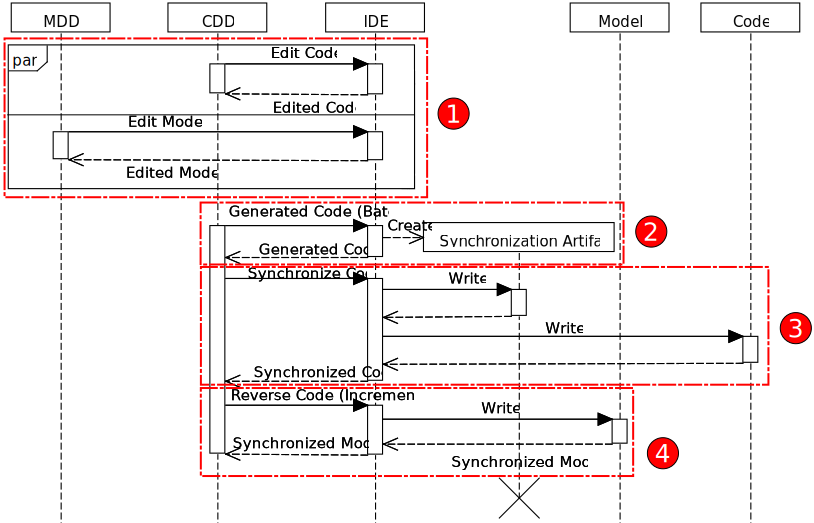
\includegraphics[width = \columnwidth]{figures/scenario3_seq}
\caption{Synchronization process, in which the model and the code are concurrently edited with code as the synchronization artifact (CDD = Code-Driven Developer, MDD = Model-Driven Developer). The API calls for Model and Code are represented generically as "Read" and "Write".}
\label{fig:scenario3}
\end{figure}

\begin{description}
	\item[Step 1] Both the model and code may be edited concurrently.
	(To simplify Figure \ref{fig:scenario3}, we don't show the Read and Write interactions for this step.)
	After both artifacts have been edited concurrently, we need to synchronize them.	
	\item[Step 2] First we create a synchronization artifact from the edited model by generating code in batch mode.
	This synchronization artifact is code and it is an image of the edited model.	
	\item[Step 3] The synchronization artifact is synchronized with the edited code. Since the synchronization artifact
is code itself, this step is done with the \texttt{Synchronize Code} use-case of the IDE.
	\item[Step 4] Once synchronization artifact and edited code are synchronized, the former is reversed incrementally to update the edited model.
\end{description}

The second strategy, based on using model as the synchronization artifact,
is the opposite of the first strategy. In the second strategy, the synchronization artifact is
obtained by reversing the edited code in batch mode.
Afterwards the synchronization artifact is synchronized with the edited model.
Finally, we generate code incrementally from the synchronization artifact to update the edited code.

%Figure \ref{fig:strategy2} shows the synchronization strategy based on using model as the synchronization artifact.
%This strategy is the opposite of the strategy presented in Figure \ref{fig:strategy1}. Its steps are described as follows:
%
%\begin{center}
%\textbf{\textit{- Steps of synchronization strategy 2 -}}
%\end{center}
%\begin{description}
%	\item[Step 1] The synchronization artifact is obtained by reversing the edited code in batch mode.
%	\item[Step 2] Afterwards the synchronization artifact is synchronized with the edited model.
%	\item[Step 3] Finally, we generate code incrementally from the synchronization artifact to update the edited code.
%\end{description}
%
%\begin{figure}
%\centering
%\includegraphics[width=\columnwidth]{figures/strategy2}
%\caption{Synchronization strategy 2 using model as synchronization artifact}
%\label{fig:strategy2}
%\end{figure}

We propose two strategies based on the preferences of the developers.
They may even use both strategies, successively, as a kind of hybrid strategy.
This may be useful
when developers want to synchronize parts of the system using one strategy,
and other parts using the other strategy. %For example, they may choose
%to synchronize method bodies using strategy 1, where the synchronization artifact is code.
%Then strategy 2, in which the synchronization artifact is a model, is used to
%to synchronize architectural elements of the system.

%In the next section we propose an implementation
%of an IDE and the proposed synchronization processes.
